\begingroup
\setlength{\abovedisplayskip}{6pt}
\setlength{\belowdisplayskip}{6pt}
\setlength{\abovedisplayshortskip}{4pt}
\setlength{\belowdisplayshortskip}{4pt}
\setlength{\intextsep}{6pt}

I take displacement $u(t)$ as positive to the right and measure it from the equilibrium position. I assume one degree of freedom, a point mass $m$, a massless linear spring with stiffness $k$, a massless viscous damper with coefficient $c$, frictionless horizontal motion, and no external force. Since the damping is nonnegative, $c\geq 0$.

The free-body diagram for the damped system is shown below. The spring force opposes displacement, and the damper force opposes velocity.

\begin{figure}[H]
\centering

\includegraphics[width=0.82\linewidth,keepaspectratio,alt={Free-body diagram for Problem B.2.}]{figures/generated/fig_pB2_fbd.pdf}
\caption{B.2.2. Free-body diagram for the damped system.}
\end{figure}

Therefore, the spring and damper forces act in the negative $x$ direction, which gives

\[
\boxed{\sum F_x=-c\dot{u}(t)-ku(t)}
\qquad\text{(B.2.2)}
\]

Applying Newton's law of motion to the mass gives

\[
\boxed{\sum F_x=m\ddot{u}(t)}
\qquad\text{(B.2.3)}
\]

Equating the force balance to the inertial force and moving all terms to the left gives the equation of motion,

\[
\boxed{m\ddot{u}(t)+c\dot{u}(t)+ku(t)=0}
\qquad\text{(B.2.4)}
\]

Since the equation is linear with constant coefficients, the nontrivial exponential trial response $u(t)=e^{st}$ applies. Its derivatives are $\dot{u}(t)=se^{st}$ and $\ddot{u}(t)=s^2e^{st}$, so substitution gives

\[
\boxed{(ms^2+cs+k)e^{st}=0}
\qquad\text{(B.2.5)}
\]

Because $e^{st}$ is never zero, the remaining factor must vanish. Thus, the characteristic equation is

\[
\boxed{ms^2+cs+k=0}
\qquad\text{(B.2.6)}
\]

Solving this quadratic equation for $s$ gives the two characteristic roots,

\[
\boxed{s_{1,2}=\frac{-c\pm\sqrt{c^2-4mk}}{2m}}
\qquad\text{(B.2.7)}
\]

Critical damping occurs when the two roots coincide. Therefore, setting the discriminant equal to zero gives

\[
c_{\mathrm{cr}}^2-4mk=0.
\]

For nonnegative damping, the critical damping value is

\[
\boxed{c_{\mathrm{cr}}=2\sqrt{mk}}
\qquad\text{(B.2.8)}
\]

The damping ratio is the physical damping divided by the critical damping. Hence,

\[
\boxed{\zeta=\frac{c}{c_{\mathrm{cr}}}=\frac{c}{2\sqrt{mk}}}
\qquad\text{(B.2.9)}
\]

Since $c\geq 0$, the three damping cases are

\[
\begin{aligned}
\boxed{0\leq\zeta<1}&\quad\text{Underdamped}\qquad\text{(B.2.10.a)}\\[2pt]
\boxed{\zeta=1}&\quad\text{Critically damped}\qquad\text{(B.2.10.b)}\\[2pt]
\boxed{\zeta>1}&\quad\text{Overdamped}\qquad\text{(B.2.10.c)}
\end{aligned}
\]

The value $\zeta=0$ is the undamped limiting case. Using $c=\zeta c_{\mathrm{cr}}$ and the critical damping expression gives the physical damping in terms of $\zeta$, $m$, and $k$,

\[
\boxed{c=2\zeta\sqrt{mk}}
\qquad\text{(B.2.11)}
\]

The stiffness-to-mass ratio is the square of the undamped natural frequency. Therefore,

\[
\boxed{\omega_n=\sqrt{\frac{k}{m}}}
\qquad\text{(B.2.12)}
\]

Using $c/(2m)=\zeta\omega_n$ and $k/m=\omega_n^2$ in the characteristic roots gives

\[
\boxed{s_{1,2}=-\zeta\omega_n\pm\omega_n\sqrt{\zeta^2-1}}
\qquad\text{(B.2.13)}
\]

For an underdamped system, $\zeta<1$, so $\zeta^2-1<0$. The square root can therefore be written as

\[
\sqrt{\zeta^2-1}=i\sqrt{1-\zeta^2}.
\]

Substitution into the roots from (B.2.13) gives the complex roots,

\[
\boxed{s_{1,2}=-\zeta\omega_n\pm i\omega_n\sqrt{1-\zeta^2}}
\qquad\text{(B.2.14)}
\]

The positive imaginary part of the underdamped roots defines the damped frequency,

\[
\boxed{\omega_d=\omega_n\sqrt{1-\zeta^2}}
\qquad\text{(B.2.15)}
\]

Substituting this definition into (B.2.14) separates the two roots as

\[
\boxed{
\begin{aligned}
s_1&=-\zeta\omega_n+i\omega_d,\\
s_2&=-\zeta\omega_n-i\omega_d.
\end{aligned}}
\qquad\text{(B.2.16)}
\]

The underdamped condition is therefore

\[
\boxed{\zeta<1}
\qquad\text{(B.2.17)}
\]

With physical nonnegative damping, this is $0\leq\zeta<1$. The value $\zeta=0$ gives the undamped limit, while $0<\zeta<1$ gives a decaying oscillation.

Using the two roots in (B.2.16), the general solution is the linear superposition of the two exponential solutions,

\[
\boxed{u(t)=C_1e^{s_1t}+C_2e^{s_2t}}
\qquad\text{(B.2.18)}
\]

Substituting the underdamped roots gives

\[
\boxed{u(t)=C_1e^{(-\zeta\omega_n+i\omega_d)t}+C_2e^{(-\zeta\omega_n-i\omega_d)t}}
\qquad\text{(B.2.19)}
\]

Because $e^{a+b}=e^ae^b$, factor out the common decay term to obtain

\[
\boxed{u(t)=e^{-\zeta\omega_nt}\left(C_1e^{i\omega_dt}+C_2e^{-i\omega_dt}\right)}
\qquad\text{(B.2.20)}
\]

Euler's identities convert the harmonic part into a real trigonometric form. With $A=C_1+C_2$ and $B=i(C_1-C_2)$,

\[
C_1e^{i\omega_dt}+C_2e^{-i\omega_dt}=A\cos(\omega_dt)+B\sin(\omega_dt).
\]

Writing this sinusoid in amplitude-phase form gives $A=C\sin\phi$ and $B=C\cos\phi$. Thus,

\[
\boxed{
u(t)=Ce^{-\zeta\omega_nt}\sin(\omega_dt+\phi),
\qquad
C=\sqrt{A^2+B^2},
\qquad
\phi=\operatorname{atan2}(A,B)
}
\qquad\text{(B.2.21)}
\]

The sinusoidal carrier is bounded by the two exponential envelopes $u_{\mathrm{env},\pm}(t)=\pm Ce^{-\zeta\omega_nt}$. The carrier keeps the constant damped frequency $\omega_d$, while its amplitude decreases with time. The resulting sketch is shown below using illustrative values $\omega_n=1$, $\zeta=0.20$, $C=1$, and $\phi=0.5$ radians.

\begin{figure}[H]
\centering
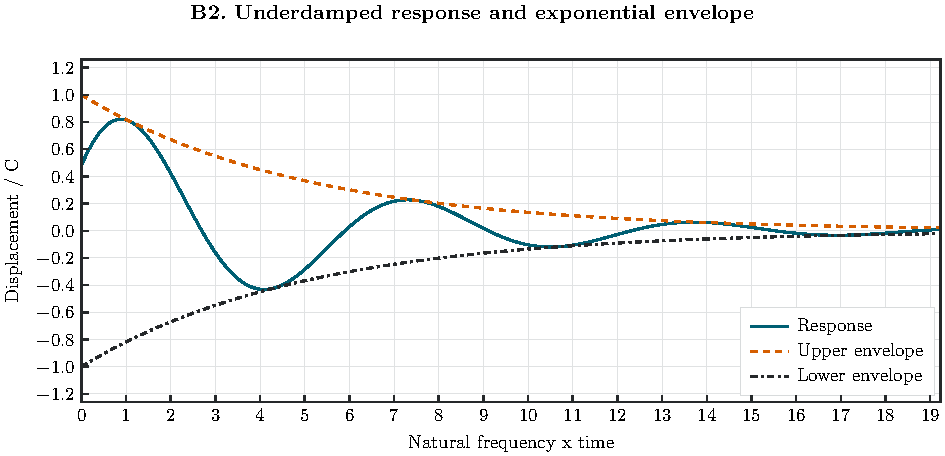
\includegraphics[width=0.95\linewidth,height=0.30\textheight,keepaspectratio,alt={Underdamped oscillation inside exponential decay envelopes.}]{figures/generated/solutions/B2_envelope.pdf}
\caption{B.2.22. Underdamped oscillation and its exponential decay envelopes.}
\end{figure}

\clearpage
\matlabcaption{Code used to reproduce the B.2.22 response sketch.}

\lstinputlisting[style=hwmatlab]{matlab/B2.m}

For the initial-displacement case, let $u(0)=u_0$ and $\dot{u}(0)=0$. Evaluating the cosine-sine form at $t=0$ gives $A=u_0$. Differentiating that form before setting $t=0$ gives

\[
\dot{u}(0)=-\zeta\omega_nA+\omega_dB=0.
\]

Therefore, $B=\zeta\omega_nu_0/\omega_d$, and the response is

\[
\boxed{u(t)=u_0e^{-\zeta\omega_nt}\left[\cos(\omega_dt)+\frac{\zeta\omega_n}{\omega_d}\sin(\omega_dt)\right]}
\qquad\text{(B.2.23)}
\]

For simultaneous initial displacement and velocity, let $u(0)=u_0$ and $\dot{u}(0)=\dot{u}_0$. The same two initial-condition equations give

\[
A=u_0,
\qquad
B=\frac{\dot{u}_0+\zeta\omega_nu_0}{\omega_d}.
\]

Substitution into the trigonometric solution gives the complete underdamped IVP response,

\[
\boxed{u(t)=e^{-\zeta\omega_nt}\left[u_0\cos(\omega_dt)+\frac{\dot{u}_0+\zeta\omega_nu_0}{\omega_d}\sin(\omega_dt)\right]}
\qquad\text{(B.2.24)}
\]

\endgroup
